\section{Magellan}
\label{sec:magellan}

\begin{frame}
  \begin{center}
    \Huge{\textcolor{red}{Magellan}}
  \end{center}
\end{frame}

\subsection{Ice Breaking}

\begin{frame}{Length Calculator}
  \begin{enumerate}
    \item \textcolor{red}{1 FEET == 12 INCH}
    \item \textcolor{red}{2 FEET != 12 INCH}
  \end{enumerate}
\end{frame}

\begin{frame}[fragile]{First Test Case}
\begin{c++}
#include "magellan/magellan.hpp"
#include "quantity/Length.h"

USING_HAMCREST_NS

FIXTURE(LengthTest)
{
    TEST("1 FEET == 12 INCH")
    {
        ASSERT_THAT(Length(1, FEET), eq(Length(12, INCH)));
    }
};
\end{c++}
\end{frame}

\begin{frame}[fragile]{include/quantity/Length.h}
\begin{c++}
#ifndef SDHS_DFJE_3747_CNDHE_37473_VNNFHEB_DHEYE
#define SDHS_DFJE_3747_CNDHE_37473_VNNFHEB_DHEYE

#include "quantity/Amount.h"
#include "quantity/LengthUnit.h"

struct Length
{
    Length(Amount amount, LengthUnit unit);

    bool operator==(const Length& rhs) const;

private:
    const Amount amountInBaseUnit;
};

#endif
\end{c++}
\end{frame}

\begin{frame}[fragile]{include/quantity/LengthUnit.h}
\begin{c++}
#ifndef ERTYT_CNNDH_ENBAW_648294_NVGDGWE_57VNDHA_CH3
#define ERTYT_CNNDH_ENBAW_648294_NVGDGWE_57VNDHA_CH3

enum LengthUnit 
{ 
    INCH = 1, 
    FEET = 12 * INCH 
};

#endif
\end{c++}
\end{frame}

\begin{frame}[fragile]{include/quantity/LengthUnit.h}
\begin{c++}
#ifndef SDFJCN_E6438C_CNDJ866_VNA001223_VNNDHHE3CHD
#define SDFJCN_E6438C_CNDJ866_VNA001223_VNNDHHE3CHD

using Amount = unsigned int;

#endif
\end{c++}
\end{frame}

\begin{frame}[fragile]{src/quantity/Length.cpp}
\begin{c++}
#include "quantity/Length.h"

Length::Length(Amount amount, LengthUnit unit)
  : amountInBaseUnit(unit * amount)
{
}

bool Length::operator==(const Length& rhs) const
{
    return amountInBaseUnit == rhs.amountInBaseUnit;
}

#endif
\end{c++}
\end{frame}

\subsection{Magellan}

\begin{frame}[fragile]{Pure OO}
\begin{c++}
FIXTURE(RobotCleanerTest)
{
    RobotCleaner robot;

    TEST("at the beginning, the robot should be in at the initial position")
    {
        ASSERT_THAT(robot.getPosition(), is(Position(0, 0, NORTH)));
    }

    TEST("the robot should be faced west after turn left")
    {
        robot.exec(left());
        ASSERT_THAT(robot.getPosition(), is(Position(0, 0, WEST)));
    }
};
\end{c++}
\end{frame}

\begin{frame}[fragile]{Extract Method}
\begin{c++}
FIXTURE(RobotCleanerTest)
{
    RobotCleaner robot;

    void WHEN_I_send_instruction(Instruction* instruction)
    {
        robot.exec(instruction);
    }

    void THEN_the_robot_cleaner_should_be_in(const Position& position)
    {
        ASSERT_THAT(robot.getPosition(), is(position));
    }

    TEST("at the beginning")
    {
        THEN_the_robot_cleaner_should_be_in(Position(0, 0, NORTH));
    }

    TEST("left instruction: 1-times")
    {
        WHEN_I_send_instruction(left());
        THEN_the_robot_cleaner_should_be_in(Position(0, 0, WEST));
    }
};
\end{c++}
\end{frame}

\begin{frame}[fragile]{Assertion and Hamcrest}
\begin{c++}
FIXTURE(StartsWithTest)
{
    TEST("case sensitive")
    {
        ASSERT_THAT("ruby-cpp", starts_with("ruby"));
        ASSERT_THAT("ruby-cpp", is(starts_with("ruby")));

        ASSERT_THAT(std::string("ruby-cpp"), starts_with("ruby"));
        ASSERT_THAT("ruby-cpp", starts_with(std::string("ruby")));
        ASSERT_THAT(std::string("ruby-cpp"), starts_with(std::string("ruby")));
    }
};
\end{c++}
\end{frame}

\begin{frame}{Matcher}
  \begin{enumerate}
    \item \textcolor{red}{anything}
    \item \textcolor{red}{eq/ne/lt/gt/le/lt}
    \item \textcolor{red}{is/is\_not}
    \item \textcolor{red}{nil}
    \item \textcolor{red}{be\_true/be\_false}
    \item \textcolor{red}{contains\_string/starts\_with/ends\_with}
    \item \textcolor{red}{close\_to/nan}
    \item \textcolor{red}{and so on...}
  \end{enumerate}
\end{frame}

\begin{frame}[fragile]{Scope of Setup/Teardown}
\begin{c++}
BEFORE_ALL("try load global configure")
{ ... }

AFTER_ALL("try load global configure")
{ ... }

FIXTURE(ObjectTest)
{
    BEFORE_CLASS()
    { ... }

    AFTER_CLASS()
    { ... }

    BEFORE()
    { ... }

    AFTER()
    { ... }
};
\end{c++}
\end{frame}

\begin{frame}[fragile]{Options}
\begin{c++}
TestOptions::TestOptions() : desc("magellan")
{
    desc.add({
        {"help,     h",   "help message"},
        {"filter,   f",   "--filter=pattern"},
        {"color,    c",   "--color=[yes|no]"},
        {"xml,      x",   "print test result into XML file"},
        {"list,     l",   "list all tests without running them"},
        {"progress, p",   "print test result in progress bar"},
        {"verbose,  v",   "verbosely list tests processed"},
        {"repeat,   r",   "how many times to repeat each test"}
    });

    // default value
    options["color"]  = "yes";
    options["repeat"] = "1";
}
\end{c++}
\end{frame}

\begin{frame}{Magellan Framework}
    \centering
    \begin{figure}
      \centering
      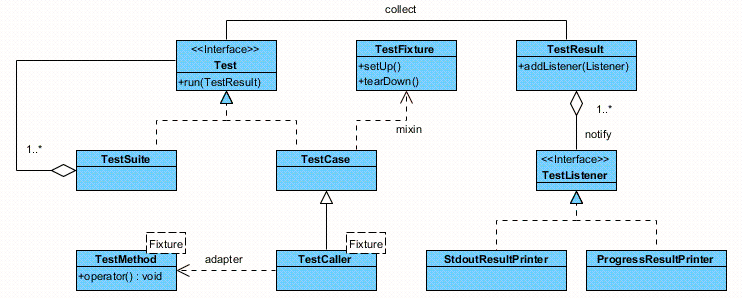
\includegraphics[width=0.95\textwidth]{magellan.png}
    \end{figure}
\end{frame}

\begin{frame}{Hamcrest Framework}
    \centering
    \begin{figure}
      \centering
      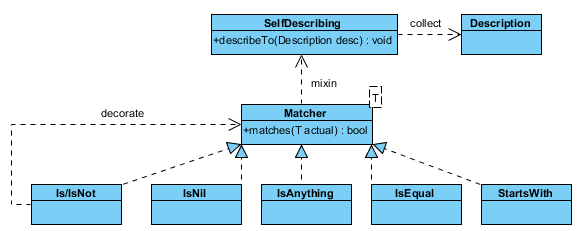
\includegraphics[width=0.8\textwidth]{hamcrest.png}
    \end{figure}
\end{frame}
